% ============================================================
%  6. MARCO TEÓRICO   (guía, 2.6)
%  Propósito: sustentar conceptualmente el proyecto.
%  CUIDADO: no debe ser una recopilación extensa de definiciones
%  desconectadas. SOLO se desarrollan conceptos que después se
%  utilizan efectivamente en el proyecto.
%  CRISP-DM: aquí se EXPLICA la metodología; su aplicación
%  práctica se documenta en el capítulo 7.
%  Transcrito de Marco_teorico.md. Las referencias "[por
%  verificar]" y las notas para el autor del .md están en
%  docs/notas_internas.md (no van en el PDF).
% ============================================================
\chapter{Marco Teórico}
\label{cap:marco-teorico}

El presente capítulo expone los fundamentos conceptuales, estadísticos y metodológicos que
sustentan el diseño del proyecto. Se organiza en cinco secciones: los fundamentos del dominio
del transporte público informal y de sus datos (\ref{sec:fundamentos-dominio}); los
fundamentos de Ciencia de Datos pertinentes a un problema de conteos espacialmente
estructurados (\ref{sec:fundamentos-cd}); las técnicas y algoritmos que integran la
comparación (\ref{sec:tecnicas-algoritmos}); las métricas con las que se evalúan
(\ref{sec:metricas}); y la metodología CRISP-DM que articula el proceso
(\ref{sec:crisp-dm}). En cada apartado se procura cerrar la exposición con la implicación
que el concepto tiene para el problema específico del proyecto, de modo que el marco teórico
funcione como justificación explícita de las decisiones metodológicas y no como una revisión
bibliográfica desconectada.

% ------------------------------------------------------------
\section{Fundamentos del dominio}
\label{sec:fundamentos-dominio}

\subsection{Transporte público informal (paratránsito) en ciudades latinoamericanas y del Sur Global}
\label{subsec:paratransito}

Se denomina transporte informal o paratránsito al conjunto de servicios de transporte de
pasajeros de tipo paratránsito que se prestan sin sanción oficial plena, generalmente con
vehículos de pequeña y mediana capacidad operados por propietarios individuales agrupados
en sindicatos, cooperativas o asociaciones \parencite{cervero2007}. En su revisión de
experiencias internacionales, \textcite{cervero2007} señalan que estos sistemas ofrecen
beneficios reales, como la movilidad a demanda para la población dependiente del transporte
público, el empleo para trabajadores de baja calificación y la cobertura de áreas carentes
de oferta formal, pero también generan costos, como congestión, contaminación atmosférica y
acústica, y accidentes de tránsito. El paratránsito no constituye, por tanto, una anomalía
marginal, sino la forma dominante de movilidad colectiva en numerosas ciudades de América
Latina, África y Asia, lo que obliga a analizarlo con herramientas propias en lugar de
asumir las categorías del transporte formal.

Uno de los rasgos que más condiciona el análisis de estos sistemas es su problema de
información. Las rutas suelen ser conocidas por los usuarios habituales, pero no están
documentadas en fuentes oficiales, y los vehículos pueden detenerse en cualquier punto del
recorrido. La propia Trufi Association describe este tipo de servicio como minibuses que
llevan a los pasajeros a su destino por rutas conocidas pero no documentadas, sin paradas
fijas, porque los pasajeros pueden subir y bajar en cualquier punto mientras haya espacio
\parencite{trufi2019}. \textcite{williams2015} constatan, para el caso de Nairobi, que en
muchas ciudades del Sur Global prácticamente no existe información digital sobre rutas,
paradas, frecuencias ni horarios de los minibuses semiformales. En Cochabamba, en
particular, no existía un archivo GTFS de transporte gestionado por la administración
pública, por lo que la información de rutas debió generarse de forma colaborativa y
publicarse como datos abiertos \parencite{osor-trufi}.

El caso de Cochabamba ilustra con claridad esta situación. \textcite{cabrera2022} sostienen
que en las ciudades bolivianas la mayor parte de los servicios de movilidad de pasajeros
pueden clasificarse como paratránsito, y caracterizan la región metropolitana de Cochabamba,
con más de 1,2~millones de habitantes en áreas urbanas de varios municipios conurbados, como
un sistema operado por centenas de organizaciones pequeñas y medianas, en el que, según una
nota del mismo artículo, cerca de 840\,000 personas realizan 2~millones de viajes diarios,
el 75~\% de ellos en el eje Sacaba-Cochabamba-Quillacollo. Según los datos que recogen estos
autores, el 55~\% de los desplazamientos se realiza en transporte público o paratránsito, el
26~\% a pie o en bicicleta, el 16~\% en vehículo privado y el 4~\% en taxi; asimismo, un
inventario realizado entre 2017 y 2020 por estudiantes de urbanismo de la Universidad Mayor
de San Simón y la Universidad Privada Boliviana identificó 132 líneas con 648 rutas
diferentes (45 de coaster, 63 de micros, 193 de taxitrufis y 347 de trufis). Los mismos
autores describen cuatro tipos de vehículo (micros, coaster, trufis y taxitrufis) y tres
formas de agencia sobre las rutas, que son la creación, la extensión y la subdivisión, a
través de las cuales la oferta acompaña, e incluso induce, la expansión urbana informal.

La implicación para el proyecto es doble. Por un lado, la ausencia de datos oficiales de
rutas convierte a la cartografía colaborativa en la única fuente sistemática de oferta, con
la consecuencia de que la cobertura observable depende del esfuerzo de mapeo y no solo de la
existencia física del servicio. Por otro lado, el carácter dinámico de las rutas, que se
crean, extienden y subdividen, implica que cualquier representación de la oferta es una
instantánea con vigencia limitada, lo que justifica un enfoque orientado a priorizar dónde
revisar la cartografía antes que a certificar su completitud.

\subsection{Cartografía colaborativa del transporte informal: OpenStreetMap, GTFS en sistemas semiformales y Trufi}
\label{subsec:cartografia-colaborativa}

OpenStreetMap (OSM) es un proyecto de cartografía abierta en el que voluntarios crean y
mantienen una base de datos geográfica mundial bajo licencia abierta \parencite{haklay2008}.
Se inscribe en el fenómeno que \textcite{goodchild2007} denominó información geográfica
voluntaria, según el cual ciudadanos sin formación cartográfica formal actúan como sensores
y productores de datos espaciales. En OSM, las líneas de transporte público se representan
mediante relaciones que agrupan las vías recorridas y, opcionalmente, las paradas, lo que
permite describir rutas de paratránsito aun cuando carezcan de paradas oficiales. La calidad
y la completitud de esta información son, sin embargo, heterogéneas en el espacio, porque
dependen de la distribución geográfica del esfuerzo voluntario.

El antecedente de referencia en la digitalización del paratránsito es el proyecto Digital
Matatus de Nairobi. \textcite{williams2015} muestran que la tecnología de telefonía celular,
ubicua en la mayoría de los países, puede emplearse para generar un conjunto de datos del
sistema semiformal de matatus en un estándar abierto, el GTFS (\textit{General Transit Feed
Specification}), concebido originalmente para el transporte formal. Los autores concluyen
que el GTFS puede adaptarse a sistemas semiformales, que existe demanda de datos
estandarizados sobre estos sistemas en los países en desarrollo y que la publicación de los
datos en un estándar abierto estimula el desarrollo de tecnologías como las aplicaciones de
ruteo. \textcite{klopp2015} complementan este trabajo con las lecciones del mismo proyecto
para el diseño de herramientas de orientación y planificación de viajes basadas en teléfonos
móviles.

En Cochabamba, esta función la cumple la Trufi Association, una organización sin fines de
lucro que desarrolla aplicaciones de movilidad para el transporte informal, que lanzó su
aplicación en Cochabamba en febrero de 2019 y que se fundó oficialmente en Hamburgo
(Alemania) en abril de ese mismo año \parencite{trufi2019}. Según la propia asociación,
desde el inicio del proyecto en abril de 2018 un equipo local recopiló más de 200 rutas de
los trufis de Cochabamba, primero en un sistema propio y luego como datos públicos en
OpenStreetMap, y en agosto de 2019 el código de la aplicación se liberó como software de
código abierto \parencite{trufi2019}. La cadena de procesamiento documentada en los
repositorios de la asociación extrae las relaciones de transporte de OSM, las convierte en
GeoJSON, genera a partir de ellas un archivo GTFS y lo carga en OpenTripPlanner para
calcular itinerarios. Versiones posteriores de la aplicación incorporaron nuevas rutas
añadidas mediante OSM y una función para que los usuarios reporten rutas faltantes o
incorrectas \parencite{trufi-v3}; la publicación de la versión~3 anuncia más de cien rutas
nuevas, mientras que otra publicación de trufi.app informa de 25 rutas nuevas con 104
conexiones nuevas, para un total de 120 rutas y 339 conexiones en Cochabamba y sus
alrededores, lo que sugiere que parte de esas cifras corresponde a conexiones y no a rutas
\parencite{trufiapp-25rutas}. La asociación informó haber superado las 20\,000 instalaciones
en Android, cerca de 30\,000 sumando las de iOS \parencite{trufi-20000}, y una publicación
posterior eleva la cifra a 100\,000 instalaciones en Android y cerca de 25\,000 en iOS, salto
que atribuye a un video de TikTok de Comteco, una cooperativa de telecomunicaciones de
Cochabamba \parencite{trufi-100000}. En su versión~5, la aplicación ofrece más de 625 rutas
mantenidas por voluntarios que mapean en OpenStreetMap, con ruteo sin conexión basado en
GTFS \parencite{trufi-v5}; la ficha de la aplicación en App Store precisa 626 rutas,
incluidas las líneas Verde y Roja y la del teleférico \parencite{trufi-appstore}.

De lo anterior se desprende que la utilidad de Trufi App en cada lugar depende directamente
de que las rutas que lo sirven hayan sido mapeadas. Una zona sin rutas cargadas no puede
producir respuestas útiles para el usuario, lo que puede desalentar su uso y reducir las
consultas; por ello, el patrón espacial de consultas contiene información sobre el esfuerzo
cartográfico, y el problema de priorizar dónde revisar o mapear rutas es, en sentido
estricto, un problema de asignación de un recurso voluntario escaso.

\subsection{El formato GTFS: estructura, trazado frente a paradas y limitaciones en sistemas informales}
\label{subsec:gtfs}

La especificación GTFS Schedule, hoy mantenida por la organización MobilityData, define un
conjunto de archivos de texto delimitados por comas que describen la oferta programada de
un sistema de transporte público \parencite{mobilitydata-gtfs}. Entre sus archivos centrales
se encuentran \var{agency.txt} (operadores), \var{routes.txt} (líneas o rutas, con su tipo
de vehículo), \var{trips.txt} (viajes concretos de cada ruta, asociados a un calendario de
servicio y, opcionalmente, a un trazado), \var{stops.txt} (paradas o puntos de acceso con sus
coordenadas), \var{stop_times.txt} (secuencia y horarios de paso de cada viaje por las
paradas) y \var{shapes.txt}, archivo opcional que describe el trazado geográfico que sigue el
vehículo mediante una secuencia ordenada de puntos (\var{shape_id}, \var{shape_pt_lat},
\var{shape_pt_lon}, \var{shape_pt_sequence}). El estándar nació de la colaboración entre la
agencia de transporte de Portland (TriMet) y Google y se convirtió en el formato de facto
para el intercambio de datos de transporte público \parencite{mchugh2013}.

Para el presente proyecto resulta fundamental distinguir entre trazado y paradas. El trazado
(\var{shapes.txt}) representa la geometría lineal por la que circula el vehículo, mientras
que las paradas (\var{stops.txt}) representan los puntos discretos en los que el estándar
supone que se produce el ascenso y el descenso. En un sistema formal ambas representaciones
coinciden en lo sustancial, porque el acceso ocurre solo en paradas. En el paratránsito
cochabambino, en cambio, el ascenso y el descenso pueden producirse a lo largo de casi todo
el recorrido, de modo que las paradas incluidas en un GTFS generado a partir de OSM son, en
gran medida, convencionales: puntos que el generador del feed ubica sobre el recorrido para
satisfacer la estructura del estándar, y no paradas reconocidas oficialmente. Medir el
acceso como distancia a esas paradas introduciría, por tanto, un artefacto del proceso de
generación del feed.

El GTFS presenta además limitaciones conocidas cuando se aplica a sistemas informales. La
primera es la vigencia: el feed es una instantánea de las rutas mapeadas en la fecha de su
generación, y las rutas del paratránsito se crean, extienden y subdividen con frecuencia
\parencite{cabrera2022}. La segunda es la naturaleza aproximada de los horarios y
frecuencias, que en ausencia de tablas oficiales se derivan de supuestos de velocidad y de
intervalos nominales. La tercera, y más relevante, es que el feed representa la oferta
mapeada y no la oferta real, porque una ruta existente pero no mapeada simplemente no
aparece. De ello se deriva que el proyecto emplea el trazado (\var{shapes.txt}) como
representación más fiel de la oferta en un sistema sin paradas fijas, y que interpreta
cualquier medida de cobertura como cobertura de la oferta conocida por Trufi App, no como
accesibilidad efectiva al transporte.

\subsection{Cobertura y accesibilidad al transporte público: ODS 11.2.1 y umbrales de caminata}
\label{subsec:ods-11-2-1}

La Agenda 2030 incorpora en su meta 11.2 el acceso a sistemas de transporte seguros,
asequibles, accesibles y sostenibles, y la monitorea mediante el indicador 11.2.1,
\enquote{proporción de la población que tiene acceso conveniente al transporte público,
desglosada por sexo, edad y personas con discapacidad}, cuyo organismo custodio es el
Programa de las Naciones Unidas para los Asentamientos Humanos (ONU-Hábitat). Según los
metadatos oficiales, actualizados el 23 de abril de 2025, el acceso se considera conveniente
cuando una parada oficialmente reconocida es accesible a una distancia a pie de 500~m,
medida a lo largo de la red vial, desde un punto de referencia como el hogar, la escuela, el
lugar de trabajo o el mercado, en el caso de sistemas de baja capacidad (por ejemplo,
autobús o BRT), o de 1~km en el caso de sistemas de alta capacidad (tren, metro,
transbordador) \parencite{onu2025}. Los metadatos añaden criterios complementarios, como la
accesibilidad para personas con necesidades especiales, la frecuencia del servicio en horas
punta y la seguridad y comodidad del entorno de la parada.

Este umbral se ha operacionalizado ampliamente con datos abiertos. El Center for
International Earth Science Information Network (CIESIN, \citeyear{ciesin2023}) calculó el
indicador para 5749 centros urbanos de 178 países, como proporción de la población de
WorldPop situada a no más de 0,5~km a pie de una parada de baja capacidad registrada en
OpenStreetMap, y oficinas estadísticas nacionales como \textcite{statcan2023} han aplicado
el mismo estándar de 500~m a lo largo de la red vial. En la literatura técnica
norteamericana, el \textit{Transit Capacity and Quality of Service Manual} (TCQSM), en su
tercera edición \parencite{tcqsm2013}, ofrece un marco para medir la disponibilidad del
transporte público desde la perspectiva del pasajero, incluida la cobertura espacial del
servicio, en el que se emplean distancias de caminata del orden de 400~m (un cuarto de
milla) para paradas de autobús y de hasta 800~m (media milla) para estaciones de modos de
alta capacidad. El rango de 400 a 800~m constituye así un intervalo de referencia razonable
para la distancia que los usuarios están dispuestos a caminar hasta el transporte público.

La adaptación de este concepto al paratránsito exige una decisión explícita. Dado que en el
sistema cochabambino el ascenso puede producirse en cualquier punto del recorrido, el
conjunto de puntos de acceso potenciales no es un conjunto de paradas, sino la propia línea
del trazado. Por ello, en el proyecto se mide la cobertura como la distancia de la zona al
trazado más cercano de las rutas del feed (\var{shapes.txt}) y se adopta el umbral de 500~m
del indicador 11.2.1 como criterio operativo de \enquote{zona cubierta}. Esta adaptación
introduce dos simplificaciones que deben declararse: se sustituye la parada oficialmente
reconocida por el trazado, y la distancia por red vial por una distancia geométrica, lo que
tiende a sobrestimar la cobertura allí donde la red vial es discontinua. El umbral es,
además, de una magnitud comparable a la arista media de una celda H3 de resolución~8
($\approx 0{,}53$~km; véase \ref{subsec:h3}), lo que hace coherente la escala de la
medida con la unidad de análisis. La cobertura así definida es un indicador de oferta
mapeada, no de accesibilidad efectiva, y su sensibilidad al umbral debe explorarse.

\subsection{Datos de consultas de una aplicación de ruteo como señal de demanda de información}
\label{subsec:consultas-senal}

La variable de interés del proyecto es el número de consultas de ruta registradas por Trufi
App, cada una caracterizada por un origen, un destino, una marca temporal y un identificador
de instalación. Conviene subrayar que una consulta no es un viaje. Una consulta expresa una
necesidad de información sobre cómo desplazarse entre dos puntos: un mismo viaje puede
generar varias consultas (por ejemplo, al comparar alternativas o repetir la búsqueda), y
muchos viajes no generan ninguna, en particular los desplazamientos habituales cuyos
usuarios ya conocen la ruta. Por ello, las consultas constituyen una señal de demanda de
información de movilidad y, solo de forma indirecta y sesgada, una señal de demanda de
viajes.

Esta señal está sujeta a varios sesgos. El primero es el de adopción: solo generan
consultas quienes tienen un teléfono inteligente, han instalado la aplicación y la usan, y
la adopción varía según el nivel socioeconómico, la edad y la exposición a campañas de
difusión; la propia Trufi Association atribuye parte del crecimiento de instalaciones al
lanzamiento de una nueva versión y a la recomendación espontánea de la creadora de
contenido de TikTok Carla Salló, con más de 1,5~millones de seguidores, tras la cual la
asociación registró un fuerte aumento de las solicitudes de itinerarios desde la aplicación
de Cochabamba \parencite{trufi-20000}. El segundo es el de necesidad de información: los
viajes poco familiares (hacia destinos nuevos, por visitantes o por trámites ocasionales)
generan proporcionalmente más consultas que los rutinarios. El tercero es el de
disponibilidad de oferta en la aplicación: si una zona no está servida por rutas mapeadas,
la aplicación no ofrece itinerarios útiles, lo que puede reducir su uso y crear un círculo
en el que la falta de cartografía y la escasez de consultas se refuerzan mutuamente.

La literatura sobre datos digitales pasivos y datos de aplicaciones como indicadores de
movilidad ha documentado ampliamente estos problemas de representatividad.
\textcite{wesolowski2013} cuantificaron, a partir de los movimientos diarios de casi
15~millones de personas en Kenia a lo largo de un año, el efecto del sesgo de tenencia de
teléfonos en las estimaciones de movilidad, y mostraron que las inferencias a nivel
poblacional se complican porque la tenencia difiere entre grupos demográficos con movilidad
distinta. \textcite{blondel2015}, en su revisión de resultados con datos de telefonía
móvil, subrayan tanto el potencial de estos datos para el análisis urbano como la necesidad
de tratar sus sesgos de cobertura. En consecuencia, las consultas de Trufi App no pueden
interpretarse como medida absoluta de la demanda de transporte, pero sí como señal relativa
cuyo nivel esperado puede modelarse en función de la población y del contexto territorial.

La implicación metodológica es que el estimando del proyecto se define explícitamente como
el número esperado de consultas, y no de viajes, de cada zona dada su población y su
contexto. En este marco, una zona poblada con cero consultas no es un dato faltante que deba
descartarse, sino una observación informativa, porque su contraste con lo esperado es
precisamente lo que puede señalar un déficit de cartografía o de adopción. Esta decisión
diferencia al proyecto del antecedente de \textcite{angulo2024}, monografía de la UMSS que
abordó la predicción de demanda en Trufi App con la metodología CRISP-DM y que excluyó las
zonas con datos insuficientes.

\subsection{Población como exposición: Kontur Population y fuentes alternativas}
\label{subsec:kontur}

La población de cada zona se toma de Kontur Population, un conjunto de datos mundial de
población distribuida en hexágonos vectoriales H3 de resolución~8 (descritos por su
productor como hexágonos de \enquote{400~m}), publicado en la plataforma Humanitarian Data
Exchange (HDX) bajo licencia Creative Commons Atribución Internacional
\parencite{kontur2023}. La ficha de HDX lo describe como una fusión depurada de datos de
GHSL, Facebook, Microsoft Buildings, Copernicus Global Land Service Land Cover, Land
Information New Zealand y OpenStreetMap, y precisa que el cálculo de la población se basa en
superponer la capa Global Human Settlement Layer (GHSL) con la población de la High
Resolution Settlement Layer (HRSL) de Facebook allí donde esta está disponible,
restringiendo con datos de OpenStreetMap los artefactos conocidos de ambas fuentes. La
documentación del productor añade que las huellas de edificios de Microsoft, los datos de
Land Information New Zealand y la cobertura del suelo de Copernicus se emplean para mejorar
la precisión de la distribución; que las canteras y las vías de gran tamaño se marcan como
no pobladas, porque GHSL las detecta a menudo erróneamente como pobladas, al igual que
lagos, ríos, glaciares, arenales y bosques; que las celdas extremadamente pobladas se
redistribuyen hacia celdas vecinas para satisfacer restricciones, preservando el total; y
que los conteos no enteros se redondean \parencite{kontur-sf}. En HDX figuran ediciones
fechadas entre el 11 de marzo de 2020 y el 1 de noviembre de 2023, entre ellas las de
2022-06-30 y 2023-11-01 que emplea el proyecto.

Kontur Population es, por tanto, una estimación modelada de tipo dasimétrico, y no un conteo
censal. Su lógica consiste en redistribuir totales de población de fuentes de base sobre la
superficie a partir de indicios de ocupación (superficie construida, edificios, cobertura
del suelo), lo que produce buenas aproximaciones agregadas pero errores locales no
despreciables en celdas individuales, sobre todo en áreas periurbanas de crecimiento
reciente o de edificación dispersa. La referencia oficial de población en Bolivia es el
Censo de Población y Vivienda 2024 del Instituto Nacional de Estadística (INE), realizado el
23 de marzo de 2024, que registró una población nacional de 11\,365\,333 habitantes
\parencite{ine2025}; en la socialización de los resultados del conteo poblacional, el INE
informó que el departamento de Cochabamba registró 2\,005\,373 habitantes
\parencite{ine2024}. Las ediciones de Kontur empleadas son anteriores a la publicación de
estos resultados censales y se apoyan en insumos de fechas previas, por lo que pueden no
reflejar plenamente la distribución de 2024; esta discrepancia temporal justifica tratar la
población como una covariable medida con error y evaluar la sensibilidad de las estimaciones
a la edición empleada.

Existen otras fuentes de población en grilla que conviene conocer para situar la elección.
WorldPop produce estimaciones de alta resolución mediante modelos de desagregación de datos
censales con bosques aleatorios alimentados por covariables geoespaciales
\parencite{stevens2015,tatem2017}, y GHS-POP, del Centro Común de Investigación de la
Comisión Europea, distribuye la población sobre la superficie construida detectada por
satélite \parencite{schiavina2023}. Las diferencias metodológicas entre estas fuentes se
traducen en discrepancias locales apreciables, por lo que ninguna puede considerarse verdad
de terreno a escala de barrio. Kontur presenta, para este proyecto, la ventaja práctica de
estar publicado de forma nativa sobre la grilla H3 de resolución~8, lo que evita una
reproyección y una reagregación adicionales.

Por último, debe distinguirse entre población residente y población flotante. Kontur estima
la población residente, es decir, dónde vive la gente, mientras que las consultas pueden
originarse también en lugares de actividad diurna (centros comerciales, mercados,
universidades, zonas de oficinas o terminales) cuya población residente es baja. En
consecuencia, en las zonas centrales o de alta actividad cabe esperar más consultas de las
que su población residente predeciría, y en zonas dormitorio la relación puede invertirse.
La implicación es que la población actúa como medida de exposición necesaria pero no
suficiente, y que las variables de contexto territorial (distancia al centro, municipio,
vecindad) cumplen la función de absorber parte de la diferencia entre población residente y
actividad efectiva.

\subsection{La lógica \texorpdfstring{\enquote{observado frente a esperado}}{"observado frente a esperado"} como instrumento de priorización}
\label{subsec:observado-esperado}

La comparación entre un conteo observado y un conteo esperado es un procedimiento clásico
de la epidemiología. La razón estandarizada de mortalidad o de morbilidad (SMR, por sus
siglas en inglés) de un área~$i$ se define como $\mathrm{SMR}_i = O_i / E_i$, donde $O_i$ es
el número de casos observados y $E_i$ el número esperado si el área tuviera las tasas de una
población de referencia; en la estandarización indirecta, $E_i = \sum_k P_{ik}\,\lambda_k$,
donde $P_{ik}$ es la población del estrato~$k$ en el área~$i$ y $\lambda_k$ la tasa de
referencia del estrato. Una razón superior a uno indica más casos de los esperados, y una
inferior, menos. La lógica es transferible a cualquier conteo cuya magnitud depende de una
población en riesgo: no interesa el conteo bruto, que refleja sobre todo el tamaño de la
población, sino su desviación respecto de lo que la población y la estructura de referencia
harían esperar.

La cartografía de enfermedades puso de relieve una dificultad central de este enfoque, el
problema de los números pequeños. \textcite{clayton1987} mostraron que, en áreas con
poblaciones pequeñas, las razones $O/E$ son muy inestables: un solo caso adicional puede
duplicar la razón, de modo que los valores extremos del mapa tienden a concentrarse en las
áreas menos pobladas por puro efecto de la varianza muestral. Su propuesta consistió en
estimadores empírico-bayesianos que contraen cada razón hacia un valor de referencia en
proporción inversa a la información disponible, y \textcite{marshall1991} desarrolló
estimadores empírico-bayesianos, globales y locales, para cartografiar tasas de enfermedad y
mortalidad con ese mismo propósito. Este problema es directamente pertinente para el
proyecto, porque un conjunto de zonas H3 de resolución~8 incluye inevitablemente zonas de
población reducida cuyas razones $O/E$ serían engañosamente extremas.

La transposición al problema de Trufi App es natural: se sustituye el caso de enfermedad
por la consulta de ruta, la población en riesgo por la población residente de la zona y la
tasa de referencia por el modelo que estima las consultas esperadas dado el contexto. La
brecha de cada zona puede expresarse en términos absolutos, $B_i = O_i - E_i$, en términos
relativos, $R_i = O_i / E_i$, o en términos probabilísticos, como la probabilidad de
observar $O_i$ o menos consultas si el verdadero valor esperado fuera $E_i$,
$p_i = P(Y \le O_i \mid \mu = E_i)$. Esta última forma incorpora la incertidumbre muestral y
mitiga el problema de los números pequeños, porque una misma razón es más significativa
cuando el valor esperado es grande. Una zona con muchas consultas esperadas y pocas
observadas se convierte así en candidata prioritaria para la revisión cartográfica.

Es imprescindible, no obstante, subrayar que la brecha orienta la revisión pero no
diagnostica por sí sola la falta de rutas. Un déficit de consultas respecto de lo esperado
puede deberse a rutas existentes pero no mapeadas, a rutas mapeadas con errores, a una baja
adopción de la aplicación en la zona, a errores en la estimación de población, a usos del
suelo no residenciales o a limitaciones del propio modelo. La brecha actúa, por tanto, como
un filtro que ordena el territorio según la magnitud de la anomalía y reduce el espacio de
búsqueda de los voluntarios, mientras que la confirmación de la causa corresponde a la
verificación cartográfica en OSM y en terreno.

% ------------------------------------------------------------
\section{Fundamentos de Ciencia de Datos}
\label{sec:fundamentos-cd}

\subsection{Ciencia de Datos y ciencia de datos geoespacial}
\label{subsec:ciencia-datos}

La Ciencia de Datos puede definirse como el campo que se ocupa de extraer conocimiento útil
de los datos mediante la integración de la estadística, la computación y el conocimiento del
dominio. \textcite{donoho2017}, en su revisión de cincuenta años de la disciplina, la
caracteriza como una ampliación de la estadística que abarca la recolección, preparación y
exploración de datos, su representación y transformación, la computación, el modelado, la
visualización y la reflexión sobre la propia práctica científica con datos.
\textcite{provost2013} subrayan, por su parte, que la Ciencia de Datos se orienta a la toma
de decisiones basada en datos, y que su valor no reside en los algoritmos en sí, sino en su
capacidad de responder preguntas bien formuladas con evidencia empírica.

Cuando los datos tienen una referencia espacial explícita, el análisis debe incorporar los
principios de la ciencia de la información geográfica (GIScience), término que
\textcite{goodchild1992} propuso para designar el estudio de las cuestiones fundamentales que
plantea el uso de la información geográfica, como la representación, la escala, la
incertidumbre y la dependencia espacial. \textcite{singleton2021} han denominado ciencia de
datos geográfica a la convergencia entre ambas tradiciones, que combina las herramientas
computacionales de la Ciencia de Datos con la atención a la estructura espacial propia de la
geografía cuantitativa. En el presente proyecto, la unidad de análisis es un lugar, la
variable de interés presenta dependencia espacial y las decisiones de escala condicionan los
resultados; por ello, el proyecto se sitúa explícitamente en el ámbito de la ciencia de
datos geoespacial y adopta sus cautelas específicas.

\subsection{Tipología del problema analítico: descriptivo, diagnóstico, predictivo y estimación transversal}
\label{subsec:tipologia-problema}

Los problemas analíticos suelen clasificarse según la pregunta que responden: el análisis
descriptivo resume lo ocurrido; el diagnóstico indaga por qué ocurrió; el predictivo estima
valores desconocidos a partir de información disponible; y el prescriptivo recomienda
acciones. Dentro del análisis predictivo conviene distinguir tres tareas que se confunden con
frecuencia. La primera es la estimación de un valor esperado condicional,
$\mu_i = E[Y_i \mid P_i, X_i]$, para unidades observadas en un mismo período, de carácter
transversal. La segunda es la proyección por escenarios, que consiste en recalcular ese valor
esperado bajo supuestos alternativos sobre las variables explicativas (por ejemplo, una nueva
distribución de la población). La tercera es el pronóstico de series temporales, que
extrapola la evolución de una variable hacia períodos futuros a partir de su dinámica pasada
\parencite{hyndman2021}.

El proyecto corresponde a la primera tarea: se estima, para cada zona, el número esperado de
consultas del período de observación dado su población y su contexto territorial, y ese
valor se contrasta con lo observado. No se pretende pronosticar cuántas consultas ocurrirán
en semanas futuras; la proyección se plantea únicamente como escenario, mediante la
actualización de la población y de los datos de consultas y la reestimación del modelo. Esta
distinción tiene una consecuencia metodológica directa: si la pregunta es cuántas consultas
cabe esperar en una zona dada su población y su contexto, la capacidad del modelo debe
evaluarse en lugares no vistos durante el entrenamiento, y no en períodos futuros. De ahí
que la validación se diseñe con particiones espaciales (véase \ref{subsec:validacion-espacial})
y no con particiones temporales.

\subsection{Datos de conteo: Poisson, exposición, sobredispersión y exceso de ceros}
\label{subsec:datos-conteo}

La variable dependiente del proyecto es un conteo, es decir, un número entero no negativo de
eventos ocurridos en una unidad espacial durante un período. El modelo de referencia para
conteos es la distribución de Poisson, cuya función de probabilidad es
\[
  P(Y = y) = \frac{e^{-\mu}\,\mu^{y}}{y!}, \qquad y = 0, 1, 2, \ldots,
\]
y cuya propiedad característica es la igualdad entre media y varianza,
$E(Y) = \operatorname{Var}(Y) = \mu$ \parencite{cameron2013}. La distribución surge
naturalmente cuando los eventos ocurren de manera independiente a una tasa constante, y
constituye el punto de partida de los modelos lineales generalizados para conteos
\parencite{mccullagh1989,agresti2015}.

Cuando las unidades difieren en tamaño, el conteo esperado es proporcional a una medida de
exposición. Si $P_i$ es la población de la zona~$i$ y $\lambda_i$ la tasa de consultas por
habitante, entonces $\mu_i = P_i \cdot \lambda_i$ y, tomando logaritmos,
$\log \mu_i = \log P_i + \log \lambda_i$. El término $\log P_i$, que entra en el modelo con
coeficiente fijo igual a uno, se denomina \textit{offset}; su inclusión garantiza que el
modelo describa tasas por habitante y que las demás variables expliquen desviaciones
respecto de la proporcionalidad con la población \parencite{cameron2013,hilbe2011}. Las
tasas suelen expresarse por cada mil habitantes, $\lambda_i \times 1000$, para facilitar su
lectura. Esta formulación es la que justifica tratar la población como exposición y no como
una variable explicativa más.

En la práctica, los conteos presentan con frecuencia una varianza superior a la media,
fenómeno denominado sobredispersión, que puede deberse a heterogeneidad no observada entre
unidades, a dependencia entre eventos o a la agregación de procesos distintos. Un
diagnóstico habitual es el estadístico de dispersión
\[
  \hat{\varphi} = \frac{1}{n - p} \sum_i \frac{(y_i - \hat{\mu}_i)^2}{\hat{\mu}_i},
\]
que en un modelo de Poisson correctamente especificado debería ser cercano a uno; valores
claramente superiores indican sobredispersión \parencite{hilbe2011}. Ignorarla no sesga
necesariamente las estimaciones puntuales, pero subestima sus errores estándar y conduce a
inferencias excesivamente confiadas \parencite{cameron2013}.

Un caso particular es el exceso de ceros, que se presenta cuando se observan más unidades
con conteo nulo de las que el modelo predice. Bajo un modelo de Poisson, el número esperado
de ceros es $\sum_i e^{-\hat{\mu}_i}$, cantidad que puede compararse con el número observado.
En el proyecto cabe esperar zonas pobladas con cero consultas, y conviene distinguir
conceptualmente entre ceros muestrales, compatibles con un valor esperado pequeño, y ceros
estructurales, que se producen porque en la zona no existe la posibilidad del evento (por
ejemplo, porque ninguna ruta mapeada la sirve y la aplicación no se usa allí). Esta
distinción motiva la consideración de modelos para sobredispersión y ceros descrita en
\ref{subsec:binomial-negativa}.

\subsection{Autocorrelación espacial: Tobler, I de Moran y LISA}
\label{subsec:autocorrelacion}

La primera ley de la geografía, formulada por \textcite{tobler1970}, establece que todo está
relacionado con todo lo demás, pero las cosas cercanas están más relacionadas que las
distantes. En términos estadísticos, esta regularidad se denomina autocorrelación espacial:
los valores de una variable en lugares próximos tienden a parecerse más (autocorrelación
positiva) o a diferir más (autocorrelación negativa) de lo que se esperaría si se
distribuyeran al azar. Su presencia viola el supuesto de independencia de las observaciones
en el que se basan muchos procedimientos estadísticos y de validación.

La medida global clásica es el índice $I$ de Moran \parencite{moran1950}, definido como
\[
  I = \frac{n}{S_0} \cdot
      \frac{\sum_i \sum_j w_{ij}\,(x_i - \bar{x})(x_j - \bar{x})}{\sum_i (x_i - \bar{x})^2},
\]
donde $n$ es el número de unidades, $x_i$ el valor en la unidad~$i$, $\bar{x}$ la media,
$w_{ij}$ el peso espacial entre las unidades $i$ y $j$, y $S_0 = \sum_i \sum_j w_{ij}$. Los
pesos se recogen en una matriz $W$ que define la vecindad. En una grilla hexagonal, la
vecindad de contigüidad resulta especialmente natural: cada zona tiene seis vecinas que
comparten con ella una arista completa (el primer anillo, obtenido en H3 con la operación
\var{grid_disk} de radio $k = 1$), de modo que $w_{ij} = 1$ si $j$ pertenece al primer
anillo de $i$ y $0$ en otro caso; habitualmente la matriz se estandariza por filas para que
cada fila sume uno. El valor esperado de $I$ bajo ausencia de autocorrelación es
$-1/(n - 1)$, y su significación se evalúa comúnmente mediante permutaciones aleatorias de
los valores entre las unidades.

Para localizar dónde se concentra la dependencia se emplean los indicadores locales de
asociación espacial (LISA) propuestos por \textcite{anselin1995}, cuya versión local del
índice de Moran es $I_i = (z_i / m_2) \sum_j w_{ij} z_j$, con $z_i = x_i - \bar{x}$ y
$m_2 = \sum_i z_i^2 / n$. La suma de los $I_i$ es proporcional al $I$ global, y cada
indicador permite clasificar las unidades en agrupamientos alto-alto y bajo-bajo, o en
atípicos alto-bajo y bajo-alto, con la debida corrección por comparaciones múltiples.
Finalmente, el correlograma espacial, que representa el valor de $I$ para vecindades de
orden creciente (anillos $k = 1, 2, 3, \ldots$), describe cómo decae la dependencia con la
distancia. En el proyecto, la autocorrelación se examina en las consultas, en las tasas y en
los residuos: el correlograma orienta la elección del tamaño de los bloques de validación
(\ref{subsec:validacion-espacial}) y el análisis de los residuos permite diagnosticar si los
modelos dejan estructura espacial sin explicar (\ref{subsec:residuos}).

\subsection{Sistemas de grillas discretas globales y H3}
\label{subsec:h3}

Un sistema de grillas discretas globales (DGGS) es una partición jerárquica de la superficie
terrestre en celdas de forma y tamaño aproximadamente regulares, a múltiples resoluciones.
\textcite{sahr2003} sistematizaron la construcción de estos sistemas geodésicos a partir de
un poliedro base, una orientación, una forma de celda, una apertura (razón de refinamiento
entre resoluciones) y una proyección entre las caras del poliedro y la esfera, y mostraron
que las grillas hexagonales basadas en el icosaedro ofrecen propiedades geométricas
favorables. H3, desarrollado originalmente por Uber y hoy mantenido como proyecto de código
abierto, es un DGGS hexagonal jerárquico construido sobre las caras de un icosaedro,
proyectadas a la esfera mediante una proyección gnomónica centrada en cada cara y orientado
de modo que sus doce vértices caen en el océano. Su resolución~0 consta de 122 celdas base
(110 hexágonos y 12 pentágonos), y cada resolución siguiente se obtiene con una apertura~7,
de modo que cada hexágono tiene siete hijos en la resolución inmediatamente más fina; en
todas las resoluciones existen exactamente 12 pentágonos, centrados en los vértices del
icosaedro \parencite{h3-overview,h3-restable}.

El hexágono presenta ventajas analíticas frente a otras teselaciones y frente a los
\textit{buffers}. A diferencia de la grilla cuadrada, en la que cada celda tiene cuatro
vecinas por arista y cuatro por vértice a distancias distintas, en la grilla hexagonal las
seis vecinas comparten una arista completa y sus centroides son equidistantes del centroide
de la celda, lo que define una vecindad uniforme y sin ambigüedad. A diferencia de los
\textit{buffers} circulares alrededor de puntos, las celdas no se solapan y cubren el
territorio de manera exhaustiva, de modo que cada evento se asigna a una sola unidad. Deben
reconocerse también sus limitaciones: la jerarquía de apertura~7 es solo aproximadamente
anidada, porque los siete hijos de un hexágono no reproducen exactamente su contorno; el
área de las celdas varía con su posición respecto de los vértices del icosaedro, con una
razón entre el hexágono de mayor y el de menor área cercana a 1,99 en la resolución~8; y los
pentágonos tienen aproximadamente la mitad del área de un hexágono de la misma resolución,
aunque, al situarse en el océano, carecen de relevancia práctica para Cochabamba
\parencite{h3-restable}.

La tabla~\ref{tab:resoluciones-h3-marco} recoge las características de las resoluciones
pertinentes para el proyecto según la tabla oficial de estadísticas de celdas de la
versión~4.x de H3. Las áreas se calculan con un modelo esférico de la Tierra basado en el
radio autálico de WGS84, y las longitudes medias de arista se calcularon exactamente para
las resoluciones 0 a 6 y se extrapolaron para las resoluciones más finas.

\begin{table}[htbp]
  \centering
  \caption{Resoluciones H3 relevantes para el proyecto}
  \label{tab:resoluciones-h3-marco}
  \interlineadoSimple
  \begin{tabularx}{\textwidth}{@{}>{\centering\arraybackslash}p{0.15\textwidth}
      >{\raggedleft\arraybackslash}p{0.14\textwidth}
      >{\raggedleft\arraybackslash}p{0.14\textwidth}
      >{\raggedleft\arraybackslash}p{0.16\textwidth}
      >{\raggedright\arraybackslash}X@{}}
    \toprule
    \textbf{Resolución} & \textbf{Área media del hexágono (km²)} &
    \textbf{Longitud media de arista (km)} & \textbf{Número total de celdas en el globo} &
    \textbf{Uso en el proyecto} \\
    \midrule
    6 & 36,1291 & 3,7245 & 14\,117\,882 & Macrozona (bloques de validación) \\
    7 & 5,1613 & 1,4065 & 98\,825\,162 & Análisis de sensibilidad (escala más gruesa) \\
    8 & 0,7373 & 0,5314 & 691\,776\,122 & Zona (unidad de análisis) \\
    9 & 0,1053 & 0,2008 & 4\,842\,432\,842 & Análisis de sensibilidad (escala más fina) \\
    \bottomrule
  \end{tabularx}
  \fuente{Elaboración propia a partir de \textcite{h3-restable}, versión 4.x.}
\end{table}

A partir de esta tabla se definen las dos unidades espaciales del proyecto. Se denomina zona
(o zona hexagonal) a la celda H3 de resolución~8, con un área media de aproximadamente
0,737~km² y una arista media de aproximadamente 0,531~km, lo que corresponde a un hexágono
de algo menos de un kilómetro entre lados opuestos, una escala asimilable a la de un barrio
urbano y coincidente con la resolución nativa de Kontur Population. Se denomina macrozona a
la celda H3 de resolución~6, con un área media de aproximadamente 36,13~km² y una arista
media de aproximadamente 3,72~km, esto es, un hexágono de unos 6,5~km entre lados opuestos,
cuya escala es asimilable a la de un distrito urbano. Dado que la apertura es~7, cada
macrozona agrupa aproximadamente $7^2 = 49$ zonas; la relación es aproximada porque la
jerarquía de H3 no está perfectamente anidada. Debe aclararse que, en este documento, el
término \enquote{zona} no corresponde a las zonas, distritos u organizaciones territoriales
de base (OTB) de la división administrativa municipal, sino exclusivamente a la celda H3 así
definida.

\subsection{Problema de la unidad de área modificable (MAUP)}
\label{subsec:maup}

El problema de la unidad de área modificable (MAUP, por sus siglas en inglés) designa la
dependencia de los resultados de un análisis espacial respecto de la forma en que se definen
las unidades de agregación \parencite{openshaw1984}. Se descompone en dos efectos: el efecto
de escala, por el cual los resultados cambian al variar el tamaño de las unidades (por
ejemplo, al agregar zonas en unidades mayores), y el efecto de zonificación, por el cual
cambian al variar la forma o la delimitación de unidades de tamaño similar.
\textcite{fotheringham1991} demostraron que los coeficientes de modelos de regresión
multivariante estimados con datos agregados pueden variar considerablemente, e incluso
cambiar de signo, según la escala y la zonificación empleadas, lo que los llevó a advertir
sobre la fiabilidad de los análisis multivariados basados en datos por área.

En el proyecto, la adopción de una grilla H3 regular y fijada de antemano reduce el
componente arbitrario de la zonificación, porque las celdas no se trazan en función de los
datos, pero no elimina el efecto de escala. Por ello, se prevé un análisis de sensibilidad a
la resolución que repite el procedimiento con celdas de resolución~7 (más gruesas) y~9 (más
finas), y que examina si la ordenación de zonas prioritarias y las conclusiones sustantivas
se mantienen al cambiar de escala. Este tratamiento no resuelve el MAUP, que carece de
solución general, pero permite informar con transparencia en qué medida las conclusiones
dependen de la resolución elegida.

\subsection{Datos faltantes y discontinuidades temporales}
\label{subsec:datos-faltantes}

\textcite{rubin1976} estableció el marco de referencia para el análisis de datos faltantes,
que distingue tres mecanismos. Los datos faltan completamente al azar (MCAR) cuando la
probabilidad de ausencia no depende ni de los valores observados ni de los no observados;
faltan al azar (MAR) cuando la probabilidad de ausencia depende solo de valores observados;
y no faltan al azar (MNAR) cuando depende de los propios valores no observados. La validez
de los métodos de tratamiento depende del mecanismo: el análisis de casos completos es
insesgado bajo MCAR, la imputación múltiple es válida bajo MAR, y bajo MNAR ningún método
resulta válido sin supuestos adicionales no verificables
\parencite{little2019,vanbuuren2018}.

Los datos de consultas del proyecto presentan un período de siete semanas consecutivas sin
registros, atribuido a un cambio en el proceso de exportación. Un mecanismo de ausencia de
origen técnico, ajeno al comportamiento de los usuarios, es plausiblemente independiente de
la zona, lo que lo aproxima a MCAR en la dimensión espacial; sin embargo, no puede
descartarse que las semanas perdidas difieran sistemáticamente de las observadas en su
dimensión temporal (por ejemplo, por estacionalidad académica o festividades). La imputación
podría, en principio, rellenar esas semanas, pero sus límites son claros: la imputación
múltiple recupera la incertidumbre solo si el modelo de imputación es adecuado
\parencite{vanbuuren2018}, y aquí no existe información auxiliar específica de esas semanas
que no esté ya contenida en las semanas observadas.

Por estas razones, en el proyecto no se generan datos sintéticos para entrenar los modelos.
Hacerlo introduciría circularidad, porque los valores imputados reproducirían el patrón del
propio modelo de imputación y el modelo posterior aprendería en parte de sí mismo; crearía
falsa precisión, porque el tamaño aparente de la muestra aumentaría sin información nueva; y
podría inducir fuga de datos, si el procedimiento de imputación empleara información de
zonas destinadas a validación o prueba. En su lugar, se normaliza el conteo por el período
efectivamente observado, expresando las consultas como tasa por semana observada
($Y_i / W_{\mathrm{obs}}$, donde $W_{\mathrm{obs}}$ es el número de semanas con registros),
y se realiza un análisis de sensibilidad que compara los resultados obtenidos con los datos
anteriores y posteriores al período sin registros. Dado que el estimando es transversal, la
ausencia de semanas afecta sobre todo al nivel global de las consultas, que la normalización
corrige, y en menor medida a su distribución espacial, que el análisis de sensibilidad
permite examinar.

\subsection{Fuga de datos}
\label{subsec:fuga-datos}

\textcite{kaufman2012} definieron la fuga de datos (\textit{data leakage}) como la
introducción, en el proceso de entrenamiento, de información sobre la variable objetivo que
no estaría legítimamente disponible en el momento de usar el modelo, lo que produce
estimaciones de desempeño optimistas que no se sostienen en la aplicación real. La fuga
puede producirse por la inclusión de variables que son consecuencia del objetivo o que lo
contienen parcialmente; por la contaminación entre los conjuntos de entrenamiento y
evaluación, por ejemplo al realizar el preprocesamiento (escalado, selección de variables,
imputación) sobre todos los datos antes de particionarlos; y por la dependencia entre
observaciones de entrenamiento y evaluación que no se respeta en la partición.
\textcite{kapoor2023}, a partir de una revisión de la literatura en campos que han adoptado
el aprendizaje automático, identificaron 17 disciplinas en las que se ha detectado fuga, que
afecta colectivamente a 294 artículos y que en algunos casos condujo a conclusiones
extremadamente optimistas; los autores propusieron una taxonomía de tipos de fuga y fichas
de información del modelo para prevenirla.

En problemas espaciales existe una forma específica de fuga que resulta crítica para este
proyecto: la que se produce en predictores construidos con información de vecinos. Una
variable como la tasa de consultas de las zonas vecinas es legítima cuando se calcula con
información disponible, pero si, al evaluar el modelo en una zona de validación, la tasa
vecinal incluye los conteos de otras zonas de validación, o de la propia zona, el modelo
accede indirectamente a la variable que debe estimar. Para evitarlo, en el proyecto las
variables basadas en la vecindad se calculan excluyendo siempre la propia zona y, dentro de
cada iteración de validación, empleando únicamente los conteos de las zonas del conjunto de
entrenamiento, de modo que ninguna información del bloque evaluado intervenga en la
construcción de sus predictores.

\subsection{Sobreajuste, compromiso sesgo-varianza y validación con estructura espacial}
\label{subsec:validacion-espacial}

Se denomina sobreajuste a la situación en la que un modelo se adapta a las particularidades
aleatorias de los datos de entrenamiento en lugar de a la estructura general del fenómeno,
de modo que su desempeño en datos nuevos es inferior al observado en entrenamiento.
\textcite{hastie2009} formalizan este fenómeno mediante la descomposición del error esperado
de predicción en un punto $x_0$,
\[
  E\bigl[(Y - \hat{f}(x_0))^2\bigr] = \sigma^2 + \bigl[\mathrm{Sesgo}(\hat{f}(x_0))\bigr]^2
    + \operatorname{Var}(\hat{f}(x_0)),
\]
donde $\sigma^2$ es el error irreducible, el sesgo refleja la incapacidad del modelo para
representar la relación verdadera y la varianza su sensibilidad a la muestra de
entrenamiento. Los modelos más flexibles reducen el sesgo a costa de aumentar la varianza, y
el objetivo de la selección de modelos es encontrar el equilibrio que minimice el error en
datos no vistos, lo que exige estimar ese error de manera honesta.

La validación cruzada aleatoria, que reparte las observaciones entre particiones al azar,
presupone que las observaciones son independientes. Cuando existe autocorrelación espacial,
las observaciones de validación tienen casi siempre vecinas muy similares en el conjunto de
entrenamiento, y el error estimado refleja la capacidad del modelo para interpolar entre
vecinos más que para generalizar a lugares nuevos. \textcite{roberts2017} mostraron que, con
datos que presentan estructura temporal, espacial, jerárquica o filogenética, la validación
aleatoria produce estimaciones de error optimistas, y recomendaron la validación por
bloques, en la que las particiones se forman con grupos de observaciones contiguas, de
tamaño acorde con el alcance de la dependencia. \textcite{valavi2019} desarrollaron el
paquete blockCV para generar particiones espacial o ambientalmente separadas, y
\textcite{ploton2020} encontraron que, al validar con puntos espacialmente independientes de
los de calibración, modelos de cartografía ecológica de gran escala que parecían muy
precisos mostraban un poder predictivo muy pobre.

Este enfoque no está exento de debate. \textcite{wadoux2021} sostienen que la validación
cruzada espacial carece de fundamento teórico como método para estimar la exactitud de un
mapa y que puede resultar pesimista, porque las particiones por bloques obligan al modelo a
extrapolar a distancias mayores que las que separan los puntos a predecir de los datos
disponibles en la aplicación real; los autores defienden el muestreo probabilístico y la
inferencia basada en el diseño como vía para obtener estimaciones insesgadas.
\textcite{meyer2022} sitúan esta controversia en el contexto más amplio de la evaluación de
mapas producidos con aprendizaje automático y subrayan que la estrategia de validación debe
corresponder a la tarea de predicción: la validación aleatoria es adecuada cuando se predice
en lugares cercanos a los datos de entrenamiento, y la validación espacial, cuando se
predice en áreas alejadas de ellos.

En el proyecto, la pregunta de interés, es decir, cuántas consultas cabe esperar en una zona
dada su población y su contexto, se aplica a zonas cuya información de consultas no debería
intervenir en su propia estimación, incluidas las zonas pobladas sin consultas. Por ello, se
adopta la validación cruzada espacial por bloques con macrozonas H3 de resolución~6 como
bloques, de modo que todas las zonas de una macrozona se asignan conjuntamente a la misma
partición, y se reconoce explícitamente que esta elección puede resultar algo pesimista. El
diseño se completa con dos salvaguardas: un conjunto de prueba reservado, formado por
macrozonas completas apartadas desde el inicio, que se utiliza una sola vez al final para
evaluar el modelo elegido; y una regla de selección declarada de antemano, basada en la
devianza de Poisson media en validación cruzada y en un criterio de parsimonia, como la
regla de un error estándar descrita por \textcite{hastie2009}, que prefiere el modelo más
simple cuyo error no difiere del mínimo en más de un error estándar. Ambas salvaguardas
impiden que la elección del modelo se ajuste, consciente o inconscientemente, al conjunto de
prueba.

% ------------------------------------------------------------
\section{Técnicas y algoritmos relacionados}
\label{sec:tecnicas-algoritmos}

Las técnicas que integran la comparación se organizan como una escalera de complejidad
creciente, que va desde líneas base de tasas, sin parámetros aprendidos más allá de
promedios, hasta modelos de aprendizaje automático no lineales. Esta estrategia se
fundamenta en el teorema de \enquote{no hay almuerzo gratis} (\textit{no free lunch}) de
\textcite{wolpert1996}, según el cual, promediado sobre todos los problemas posibles, ningún
algoritmo de aprendizaje supera a otro, de modo que la superioridad de una técnica solo
puede establecerse empíricamente para una clase de problemas concreta. En consecuencia, la
práctica recomendada consiste en comparar los modelos complejos con líneas base simples e
interpretables: si un modelo sofisticado no mejora de manera sustantiva a una tasa
proporcional a la población, su complejidad adicional no está justificada. Cada peldaño de
la escalera responde a una hipótesis distinta sobre qué información explica las consultas
esperadas, y su inclusión se justifica en esos términos.

\subsection{Líneas base de tasas: tasa global y tasas estratificadas}
\label{subsec:lineas-base}

La línea base más simple supone que las consultas son proporcionales a la población, con
una tasa común a todo el territorio. La tasa global se estima como
$\hat{\lambda} = \sum_i Y_i / \sum_i P_i$, y las consultas esperadas de cada zona como
$\hat{\mu}_i = \hat{\lambda} \cdot P_i$. Este modelo encarna la hipótesis nula sustantiva
del proyecto, según la cual la población basta para explicar las consultas, y constituye por
ello el modelo de referencia contra el que se miden todos los demás (véase
\ref{subsec:modelo-referencia}).

Un primer refinamiento consiste en estratificar la tasa. Si $g(i)$ denota el estrato al que
pertenece la zona~$i$, la tasa del estrato se estima como
$\hat{\lambda}_g = \sum_{i \in g} Y_i / \sum_{i \in g} P_i$, y las consultas esperadas como
$\hat{\mu}_i = \hat{\lambda}_{g(i)} \cdot P_i$. Este procedimiento es análogo a la
estandarización de tasas por estratos empleada en demografía y epidemiología, y permite
incorporar heterogeneidad sin estimar modelos. En el proyecto se consideran dos
estratificaciones: por municipio, que captura diferencias institucionales, de adopción o de
cobertura cartográfica entre los municipios del eje metropolitano, y por anillos de
distancia al centro, que captura el gradiente centro-periferia.

La estratificación por anillos se fundamenta en la economía urbana, cuyos modelos clásicos
de localización, como el de \textcite{alonso1964}, predicen que la intensidad de uso del
suelo y la densidad disminuyen con la distancia al centro de negocios, y cuyos estudios
empíricos, desde \textcite{clark1951}, han descrito la densidad de población urbana como una
función aproximadamente exponencial negativa de esa distancia. Por analogía, cabe esperar
que la tasa de consultas por habitante también varíe con la distancia al centro, ya sea por
la concentración de actividades y destinos, por diferencias socioeconómicas en la adopción
de la aplicación o por la desigual densidad de rutas mapeadas. Las líneas base
estratificadas permiten examinar si esta estructura simple explica una parte sustancial de
la variación antes de recurrir a modelos más complejos.

\subsection{Suavizado espacial por vecindad}
\label{subsec:suavizado-vecindad}

El segundo peldaño aprovecha la autocorrelación espacial mediante un estimador de suavizado
local. Para cada zona~$i$, con primer anillo de vecinas $N(i)$, que excluye a la propia
zona, las consultas esperadas se estiman como
\[
  \hat{\mu}_i = P_i \cdot \frac{\sum_{j \in N(i)} Y_j}{\sum_{j \in N(i)} P_j},
\]
es decir, la población de la zona multiplicada por la tasa conjunta de sus vecinas. El
estimador encarna la hipótesis de que zonas próximas comparten las condiciones que
determinan la tasa de consultas, como la adopción, la cobertura cartográfica o el perfil
socioeconómico, en coherencia con la primera ley de Tobler.

Este estimador se relaciona con dos familias de métodos. Por una parte, con los estimadores
empírico-bayesianos de tasas: \textcite{clayton1987} y \textcite{marshall1991} propusieron
contraer la tasa bruta de cada área hacia una tasa de referencia, global o local, con un
peso que aumenta cuando la población del área es pequeña, y el suavizado local por vecindad
puede interpretarse como el caso límite en el que la tasa propia recibe peso nulo y la tasa
vecinal peso total; programas de análisis espacial como GeoDa han difundido estos suavizados
de tasas en la práctica aplicada \parencite{anselin2006}. Por otra parte, se relaciona con
la regresión por vecinos más cercanos, en la que la predicción de una unidad se obtiene como
promedio de las respuestas de las unidades más próximas; aquí la proximidad se define por
contigüidad hexagonal y el promedio se pondera por la población.

La aplicación de este estimador requiere cuidados específicos para evitar la fuga descrita
en \ref{subsec:fuga-datos}. La tasa vecinal debe calcularse sin incluir la propia zona y, en
cada iteración de validación, solo con las zonas del conjunto de entrenamiento; las zonas
cuyo primer anillo queda íntegramente fuera del entrenamiento, situación frecuente en el
interior de los bloques de validación, requieren una regla de respaldo declarada de
antemano, como recurrir al segundo anillo o a la tasa global. Estas precauciones garantizan
que el suavizado se evalúe en las mismas condiciones en las que se aplicaría a una zona cuyas
consultas no se conocen.

\subsection{Modelos lineales generalizados: regresión de Poisson con offset}
\label{subsec:glm-poisson}

Los modelos lineales generalizados (GLM), introducidos por \textcite{nelder1972} y
desarrollados sistemáticamente por \textcite{mccullagh1989}, extienden la regresión lineal a
variables respuesta de la familia exponencial mediante tres componentes: una distribución
para la respuesta, un predictor lineal $\eta_i = x_i^{\top}\beta$ y una función de enlace $g$
que relaciona la media con el predictor, $g(\mu_i) = \eta_i$. La regresión de Poisson
corresponde a la distribución de Poisson con enlace logarítmico. Incorporando la población
como exposición, el modelo se escribe $\log \mu_i = \log P_i + \beta_0 + x_i^{\top}\beta$, o
de manera equivalente $\mu_i = P_i \cdot \exp(\beta_0 + x_i^{\top}\beta)$, lo que en notación
compacta se expresa como $\log \mu = \log P + X\beta$. Los parámetros se estiman por máxima
verosimilitud mediante mínimos cuadrados reponderados iterativamente
\parencite{nelder1972}.

La principal ventaja de este peldaño es su interpretabilidad: cada coeficiente representa el
cambio en el logaritmo de la tasa de consultas por habitante asociado a una unidad de la
variable correspondiente, de modo que $\exp(\beta_k)$ es una razón de tasas. Por ejemplo, un
coeficiente asociado a la cobertura se interpretaría como el factor multiplicativo de la tasa
en las zonas cubiertas respecto de las no cubiertas, manteniendo constantes las demás
variables. En términos de implementación, la biblioteca statsmodels admite directamente un
\textit{offset} en sus modelos GLM, mientras que en scikit-learn, cuyo
\var{PoissonRegressor} no admite \textit{offset}, puede obtenerse un ajuste equivalente
modelando la tasa $y_i / P_i$ con pesos muestrales iguales a $P_i$. Este modelo encarna la
hipótesis de que las variables de contexto actúan de forma multiplicativa y aditiva en la
escala logarítmica, sin interacciones no especificadas.

\subsection{Regresión binomial negativa y modelos con exceso de ceros}
\label{subsec:binomial-negativa}

Cuando existe sobredispersión, la regresión binomial negativa ofrece una generalización
natural de la de Poisson. En su parametrización más común, denominada NB2, la media conserva
la misma estructura, $\log \mu_i = \log P_i + x_i^{\top}\beta$, pero la varianza pasa a ser
$\operatorname{Var}(Y_i) = \mu_i + \alpha \mu_i^2$, donde $\alpha \ge 0$ es el parámetro de
dispersión; cuando $\alpha$ tiende a cero, el modelo se reduce al de Poisson
\parencite{hilbe2011,cameron2013}. La binomial negativa puede derivarse como una mezcla de
Poisson con heterogeneidad no observada de distribución gamma, lo que le confiere una
interpretación sustantiva: zonas con las mismas características observadas pueden diferir en
factores no medidos, como la intensidad de difusión local de la aplicación. Su inclusión en
la comparación se justifica porque, ante sobredispersión, ofrece errores estándar más
realistas y pondera de forma distinta las zonas de conteos altos.

Cuando el exceso de ceros persiste incluso tras considerar la sobredispersión, pueden
emplearse modelos inflados de ceros, que combinan un proceso binario que genera ceros
estructurales con probabilidad~$\pi$ y un proceso de conteo, de modo que
$P(Y = 0) = \pi + (1 - \pi) \cdot f(0; \mu)$ \parencite{lambert1992}, o modelos de valla
(\textit{hurdle}), que separan la decisión de si hay o no eventos de la cantidad de eventos
cuando los hay. La decisión entre estas alternativas no debe basarse en un único contraste
mecánico, sino en la combinación de varios criterios: la comparación entre el número de
ceros observados y el esperado bajo el modelo binomial negativo, los criterios de
información y el desempeño en validación, y la plausibilidad sustantiva de un proceso
generador de ceros estructurales. Conviene recordar que la binomial negativa, por su mayor
varianza, predice más ceros que la Poisson con la misma media, por lo que con frecuencia
absorbe buena parte del aparente exceso de ceros.

\subsection{Gradient boosting con pérdida de Poisson}
\label{subsec:gradient-boosting}

El \textit{gradient boosting}, formalizado por \textcite{friedman2001}, construye un modelo
aditivo $F(x) = \sum_m \nu \cdot h_m(x)$ mediante la incorporación secuencial de aprendices
débiles, normalmente árboles de decisión poco profundos, cada uno ajustado al gradiente
negativo de la función de pérdida respecto de las predicciones del modelo acumulado, con una
tasa de aprendizaje~$\nu$ que controla la contribución de cada árbol. Su atractivo para el
proyecto reside en que captura relaciones no lineales e interacciones entre variables sin
necesidad de especificarlas de antemano, algo que un GLM solo logra si el analista las
introduce explícitamente. Cuando la pérdida es la devianza de Poisson y el enlace es
logarítmico, el modelo estima directamente el logaritmo del conteo esperado, conservando la
coherencia con la naturaleza de los datos.

Existen varias implementaciones eficientes. XGBoost \parencite{chen2016} introdujo un
objetivo regularizado, un algoritmo de búsqueda de cortes consciente de la dispersión de los
datos y optimizaciones de sistema que lo convirtieron en referencia en la práctica; ofrece
el objetivo \var{count:poisson} y permite incorporar la exposición como margen base
(\var{base_margin}) igual a $\log P_i$. LightGBM \parencite{ke2017} acelera el entrenamiento
mediante el muestreo de observaciones basado en gradientes y la agrupación de variables
mutuamente excluyentes, ofrece un objetivo de Poisson y admite la exposición como puntuación
inicial (\var{init_score}). En scikit-learn, \var{HistGradientBoostingRegressor}, basado en
histogramas, admite \var{loss="poisson"} desde la versión 0.23; según la documentación
oficial, esta pérdida implementa internamente la mitad de la devianza de Poisson con enlace
logarítmico y requiere $y \ge 0$ \parencite{sklearn-hgb}. Como este estimador no admite
\textit{offset}, la exposición puede incorporarse modelando la tasa $y_i / P_i$ con pesos
muestrales $P_i$, formulación equivalente en esperanza a la del \textit{offset}.

La flexibilidad del \textit{gradient boosting} implica un mayor riesgo de sobreajuste, por
lo que su uso requiere controlar hiperparámetros como el número de iteraciones, la
profundidad o el número de hojas de los árboles, la tasa de aprendizaje y la
regularización, idealmente mediante parada temprana y búsqueda de hiperparámetros dentro de
la propia validación cruzada espacial, sin tocar el conjunto de prueba. Su menor
interpretabilidad puede compensarse parcialmente con gráficos de dependencia parcial. Este
peldaño encarna la hipótesis de que la relación entre contexto y tasa de consultas es no
lineal o presenta interacciones relevantes, y su inclusión permite verificar empíricamente
si esa complejidad adicional se traduce en una mejora sobre modelos más simples.

\subsection{Preparación de variables geoespaciales}
\label{subsec:preparacion-geoespacial}

La construcción del conjunto de datos analítico requiere varias operaciones geoespaciales.
La primera es la asignación de cada consulta a una zona, que se realiza convirtiendo las
coordenadas de origen (latitud y longitud en WGS84) al identificador de la celda H3 de
resolución~8 que las contiene, mediante la función \var{latlng_to_cell} de la biblioteca H3
en su versión~4.x; la misma operación, aplicada a otras resoluciones, genera las variantes de
sensibilidad, y la función que devuelve la celda padre de resolución~6 asigna cada zona a su
macrozona. Previamente, las consultas se depuran de registros con coordenadas inválidas o
situadas fuera del área de estudio y de posibles repeticiones de la misma consulta por un
mismo identificador de instalación en intervalos muy breves, y se agregan los conteos por
zona.

La segunda operación es la integración con la población y con la oferta. Dado que Kontur
Population se publica sobre la misma grilla H3 de resolución~8, la unión con las zonas se
realiza por identificador de celda, sin pérdida por reproyección; para otras resoluciones,
la población se agrega sumando las celdas hijas o se reparte según corresponda. La cobertura
se calcula como la distancia mínima entre la geometría de la zona (o su centroide) y los
trazados del feed GTFS reconstruidos como líneas a partir de \var{shapes.txt}. Estas
distancias deben calcularse en un sistema de coordenadas proyectado métrico, como la
proyección UTM zona 19~Sur (EPSG:32719) que corresponde a Cochabamba, y no en grados
geográficos. Las uniones espaciales (\textit{spatial joins}) de GeoPandas permiten además
asignar a cada zona el municipio en el que se sitúa la mayor parte de su superficie.

La tercera operación es la construcción de las variables de contexto: la distancia del
centroide de la zona al centro de la ciudad y su discretización en anillos; el municipio; el
indicador de cobertura según el umbral de 500~m y la distancia continua al trazado; y las
variables de vecindad, como la población del primer anillo o la tasa vecinal calculada con
las precauciones contra la fuga descritas en \ref{subsec:fuga-datos}. Todas estas
transformaciones se implementan como funciones reproducibles que se ajustan, cuando tienen
parámetros dependientes de los datos, solo con las zonas de entrenamiento de cada
iteración.

\subsection{Entorno tecnológico}
\label{subsec:entorno-tecnologico}

El proyecto se desarrolla en Python, lenguaje que concentra el ecosistema de bibliotecas
abiertas más amplio para la Ciencia de Datos y el análisis geoespacial. La manipulación de
datos tabulares se realiza con pandas \parencite{mckinney2010}, y la de datos geoespaciales
vectoriales con GeoPandas \parencite{jordahl2020}, que extiende pandas con geometrías y
operaciones espaciales como las uniones y los cálculos de distancia. La indexación en la
grilla hexagonal se efectúa con h3-py, el enlace oficial para Python de la biblioteca H3
\parencite{h3-overview}. El análisis de autocorrelación espacial, incluidos el $I$ de Moran,
los indicadores LISA y la construcción de matrices de pesos, se realiza con PySAL y su
módulo esda \parencite{rey2007}.

Para el modelado se emplean scikit-learn \parencite{pedregosa2011}, que proporciona los
estimadores de \textit{gradient boosting} basados en histogramas, las utilidades de
validación cruzada por grupos y las métricas de devianza; statsmodels
\parencite{seabold2010}, que ofrece los modelos lineales generalizados de Poisson y binomial
negativa con \textit{offset} e inferencia estadística completa; y, de forma complementaria,
XGBoost \parencite{chen2016} y LightGBM \parencite{ke2017}. Los mapas interactivos de
estimaciones y brechas se generan con Folium, biblioteca que produce mapas web basados en
Leaflet \parencite{folium}. La reproducibilidad se asegura fijando las versiones de las
bibliotecas y las semillas aleatorias, y organizando el código como una secuencia de guiones
que puede reejecutarse de principio a fin.

% ------------------------------------------------------------
\section{Métricas de evaluación}
\label{sec:metricas}

\subsection{Modelo de referencia}
\label{subsec:modelo-referencia}

Toda evaluación de modelos requiere un punto de comparación, porque ninguna métrica de error
tiene sentido en términos absolutos: una devianza o un error medio solo son grandes o
pequeños en relación con lo que lograría una alternativa razonable, y dependen de la escala
de los conteos, del número de zonas y de la dispersión intrínseca de los datos. En el
proyecto, el modelo de referencia es la tasa global proporcional a la población descrita en
\ref{subsec:lineas-base}, $\hat{\mu}_i = \hat{\lambda} \cdot P_i$. Su elección no es
arbitraria, sino que materializa la pregunta del proyecto: si un modelo no mejora esta
referencia, el contexto territorial no aporta información sobre las consultas esperadas más
allá de la población, y la brecha observado-esperado se reduce a una comparación de tasas
brutas. Todas las métricas se reportan, por tanto, junto con su valor para el modelo de
referencia y, cuando procede, como mejora relativa respecto de él.

\subsection{Devianza de Poisson}
\label{subsec:devianza-poisson}

La devianza de Poisson mide la discrepancia entre los conteos observados y los esperados en
la escala natural de los datos de conteo. Se define como
\[
  D = 2 \sum_i \left[ y_i \ln\!\left(\frac{y_i}{\hat{\mu}_i}\right) - (y_i - \hat{\mu}_i) \right],
\]
con la convención de que $y_i \ln(y_i / \hat{\mu}_i) = 0$ cuando $y_i = 0$, y la devianza
media como $D / n$. Equivale al doble de la diferencia entre la log-verosimilitud del modelo
saturado y la del modelo evaluado, por lo que constituye la medida de ajuste natural de los
modelos de Poisson \parencite{mccullagh1989}. En scikit-learn, la función
\var{mean_poisson_deviance} calcula la devianza media y equivale a la devianza de Tweedie
con parámetro de potencia igual a uno; requiere $y \ge 0$ y predicciones estrictamente
positivas \parencite{sklearn-mpd}.

La preferencia por la devianza de Poisson frente al error absoluto medio (MAE) o a la raíz
del error cuadrático medio (RMSE) obedece a la heterogeneidad de escala de los conteos. En un
conjunto de zonas con conteos que van desde cero hasta valores elevados, el RMSE queda
dominado por los errores de las pocas zonas con muchas consultas, mientras que la devianza
de Poisson pondera cada error en relación con la magnitud esperada, en coherencia con la
propiedad de que la varianza de un conteo crece con su media. Además, la devianza de Poisson
es una función de pérdida estrictamente consistente para la media, en el sentido de
\textcite{gneiting2011}: su valor esperado se minimiza cuando la predicción coincide con el
verdadero valor esperado, que es precisamente el estimando del proyecto. El MAE, en cambio,
es consistente para la mediana, que en conteos pequeños y asimétricos puede diferir
notablemente de la media.

\subsection{Fracción de devianza explicada (\texorpdfstring{$D^2$}{D²})}
\label{subsec:d2}

La fracción de devianza explicada, o $D^2$, es el análogo del coeficiente de determinación
$R^2$ para modelos de conteo, y se define como
$D^2 = 1 - D_{\mathrm{modelo}} / D_{\mathrm{nulo}}$, donde $D_{\mathrm{nulo}}$ es la devianza
de un modelo nulo de comparación. Un valor de uno indica ajuste perfecto, un valor de cero
indica que el modelo no mejora al nulo, y un valor negativo indica que es peor. En
scikit-learn, la función \var{d2_tweedie_score} con parámetro de potencia igual a uno calcula
esta fracción tomando como modelo nulo la media constante de los valores observados; como en
el caso del $R^2$, la puntuación puede ser negativa \parencite{sklearn-d2}.

La interpretación del $D^2$ exige declarar contra qué modelo nulo se compara, porque su valor
cambia radicalmente según la elección. Frente a una media constante, que asigna el mismo
número de consultas a todas las zonas con independencia de su población, cualquier modelo
que incorpore la población obtendrá un $D^2$ elevado, sin que ello revele valor alguno del
contexto territorial. Frente al modelo de referencia con población, el $D^2$ mide la mejora
atribuible al contexto. Por ello, en el proyecto se reportan ambos valores de forma
explícita y se añade la mejora relativa frente al modelo de referencia,
$\mathrm{MR} = 1 - D_{\mathrm{modelo}} / D_{\mathrm{referencia}}$, que expresa qué fracción
de la devianza no explicada por la tasa global logra reducir cada técnica.

\subsection{Calibración}
\label{subsec:calibracion}

Un modelo puede ordenar bien las zonas y, sin embargo, sobrestimar o subestimar
sistemáticamente el nivel de las consultas. La calibración global se evalúa mediante el
cociente $C = \sum_i \hat{\mu}_i / \sum_i y_i$, que debe ser cercano a uno; los modelos de
Poisson con intercepto ajustados por máxima verosimilitud satisfacen esta igualdad en los
datos de entrenamiento, pero no necesariamente en datos no vistos. La calibración por
deciles complementa esta medida: se ordenan las zonas según su valor predicho, se agrupan en
diez grupos de igual tamaño y se compara, en cada grupo, la media de las consultas predichas
con la media de las observadas. La representación gráfica de estos pares frente a la
diagonal permite detectar si el modelo sobrestima las zonas de baja demanda esperada o
subestima las de alta demanda, patrones que afectarían directamente a la ordenación de las
brechas.

\subsection{Residuos para conteos}
\label{subsec:residuos}

El análisis de residuos permite diagnosticar dónde y cómo falla un modelo. El residuo de
Pearson se define como $r_{P,i} = (y_i - \hat{\mu}_i) / \sqrt{V(\hat{\mu}_i)}$, donde
$V(\mu)$ es la función de varianza del modelo, igual a $\mu$ en la Poisson y a
$\mu + \alpha\mu^2$ en la binomial negativa; la suma de sus cuadrados, dividida por los
grados de libertad residuales, proporciona el estadístico de dispersión de
\ref{subsec:datos-conteo}. El residuo de devianza se define como
$r_{D,i} = \operatorname{signo}(y_i - \hat{\mu}_i) \cdot \sqrt{d_i}$, con
$d_i = 2\left[y_i \ln(y_i / \hat{\mu}_i) - (y_i - \hat{\mu}_i)\right]$, de modo que la suma
de sus cuadrados es la devianza total \parencite{mccullagh1989}. Los residuos de devianza
tienen, en general, una distribución más próxima a la simétrica que los de Pearson, lo que
facilita su inspección visual.

En un contexto espacial, los residuos deben examinarse también en el mapa. La
representación cartográfica de los residuos de las zonas de validación permite identificar
áreas en las que el modelo sobrestima o subestima de forma sistemática, y el cálculo del $I$
de Moran y de los indicadores LISA sobre los residuos permite diagnosticar si persiste
autocorrelación espacial no explicada \parencite{anselin1995}. Una autocorrelación residual
significativa indica que falta en el modelo alguna variable con estructura espacial y, en el
contexto del proyecto, puede señalar agrupamientos de zonas con déficit de consultas
compatibles con áreas enteras de cartografía incompleta, información sustantiva para la
priorización.

\subsection{Estabilidad de la priorización}
\label{subsec:estabilidad-priorizacion}

Dado que el producto final del proyecto es una ordenación de zonas para su revisión, importa
tanto la exactitud de las estimaciones como la estabilidad de esa ordenación frente a
decisiones metodológicas razonables. La correlación de rangos de Spearman
\parencite{spearman1904} mide la concordancia entre dos ordenaciones, y en ausencia de
empates se calcula como
\[
  \rho = 1 - \frac{6 \sum_i d_i^2}{n(n^2 - 1)},
\]
donde $d_i$ es la diferencia entre los rangos de la zona~$i$ en ambas ordenaciones y $n$ el
número de zonas. Un valor cercano a uno indica que las dos variantes ordenan las zonas de
forma casi idéntica.

Como la priorización se concentra en el extremo superior de la lista, la correlación de
rangos, que pondera por igual todo el ordenamiento, se complementa con una medida de
solapamiento del conjunto de zonas priorizadas. Si $A$ y $B$ son los conjuntos de las $k$
zonas con mayor prioridad bajo dos variantes, el índice de Jaccard
$J = \lvert A \cap B \rvert / \lvert A \cup B \rvert$ mide la proporción de zonas
compartidas. En el proyecto, estas medidas se calculan entre las variantes que surgen de las
decisiones metodológicas documentadas: las dos ediciones de Kontur Population (2022-06-30 y
2023-11-01), las resoluciones H3 7, 8 y 9 (comparadas tras agregar las prioridades a una
escala común) y los períodos anterior y posterior al hueco de siete semanas.

\subsection{Comparación de grupos con y sin cobertura}
\label{subsec:comparacion-cobertura}

Para describir si las zonas cubiertas por el trazado de las rutas difieren de las no
cubiertas en su tasa de consultas o en su brecha, se emplea la prueba de Mann-Whitney
\parencite{mann1947}, una prueba no paramétrica que no supone normalidad y que contrasta si
los valores de un grupo tienden a ser mayores que los del otro. Su estadístico $U$ cuenta el
número de pares, formados por una observación de cada grupo, en los que la del primer grupo
supera a la del segundo, y resulta adecuado para distribuciones asimétricas con abundancia de
ceros como las de este proyecto.

La significación estadística se complementa con un tamaño de efecto. El $\delta$ de Cliff
\parencite{cliff1993} se define como
\[
  \delta = \frac{\#(x_i > y_j) - \#(x_i < y_j)}{n_1 \cdot n_2},
\]
es decir, la diferencia entre la proporción de pares en los que el primer grupo supera al
segundo y la proporción en que ocurre lo contrario; toma valores entre $-1$ y $1$ y se
relaciona con el estadístico de Mann-Whitney mediante $\delta = 2U / (n_1 n_2) - 1$. Para su
interpretación se emplean los umbrales de \textcite{romano2006}: efecto despreciable si
$\lvert\delta\rvert < 0{,}147$, pequeño si $\lvert\delta\rvert < 0{,}33$, mediano si
$\lvert\delta\rvert < 0{,}474$ y grande en caso contrario. Debe advertirse que, con
autocorrelación espacial, las observaciones no son independientes y el tamaño efectivo de la
muestra es menor que el nominal, de modo que los $p$-valores de la prueba de Mann-Whitney
resultan optimistas; por ello, en el proyecto se privilegia la magnitud del efecto frente a
la significación, y la comparación se interpreta como descriptiva, no como prueba causal del
efecto de la cobertura.

\subsection{Evaluación desagregada y análisis de sensibilidad}
\label{subsec:evaluacion-desagregada}

Una métrica global puede ocultar desempeños muy desiguales entre subconjuntos del
territorio. Por ello, las métricas de \ref{subsec:devianza-poisson} a
\ref{subsec:calibracion} se calculan también de forma desagregada: por anillos de distancia
al centro, para verificar si el modelo funciona igual en el centro que en la periferia; por
municipio, para detectar si alguno queda sistemáticamente mal representado; y por niveles de
población (por ejemplo, terciles), para examinar el comportamiento en las zonas menos
pobladas, donde el problema de los números pequeños es más agudo. Un modelo cuya ventaja
global se concentre en un solo estrato, o que empeore en las zonas periféricas donde la
priorización es más necesaria, debe interpretarse con cautela.

El análisis de sensibilidad completa la evaluación examinando la robustez de las
conclusiones frente a las decisiones metodológicas que no pueden fijarse con certeza: la
edición de la población, la resolución de la grilla, el umbral de cobertura, el período de
datos respecto del hueco de siete semanas y, en su caso, el tamaño de los bloques de
validación. Su propósito no es elegir la variante más favorable, sino documentar qué
conclusiones se mantienen bajo todas las variantes razonables y cuáles dependen de supuestos
particulares, información indispensable para que los voluntarios interpreten la lista de
zonas prioritarias con el grado de confianza adecuado.

% ------------------------------------------------------------
\section{Metodología CRISP-DM}
\label{sec:crisp-dm}

CRISP-DM (\textit{Cross-Industry Standard Process for Data Mining}) es un modelo de proceso
para proyectos de minería de datos, desarrollado a finales de la década de 1990 por un
consorcio de empresas en el marco de un proyecto financiado por la Unión Europea y publicado
como guía de referencia en su versión~1.0 \parencite{chapman2000}. Su propósito es ofrecer
un marco independiente de la industria, de la herramienta y de la aplicación, que haga los
proyectos más fiables, repetibles, manejables y menos costosos \parencite{wirth2000}. El
modelo organiza el ciclo de vida del proyecto en seis fases: comprensión del negocio, en la
que se definen los objetivos y requisitos desde la perspectiva de la organización y se
traducen en un problema analítico; comprensión de los datos, que comprende la recolección
inicial, la descripción, la exploración y la verificación de la calidad; preparación de los
datos, que abarca la selección, limpieza, construcción, integración y formateo del conjunto
de datos final; modelado, en el que se seleccionan y aplican las técnicas y se calibran sus
parámetros; evaluación, en la que se valora si los modelos satisfacen los objetivos del
negocio y se revisa el proceso; y despliegue, en el que el conocimiento obtenido se organiza
y presenta de forma que la organización pueda utilizarlo, incluyendo la planificación del
monitoreo y el mantenimiento \parencite{chapman2000}.

\begin{figure}[htbp]
  \centering
  \caption{Fases de la metodología CRISP-DM}
  \label{fig:crisp-dm}
  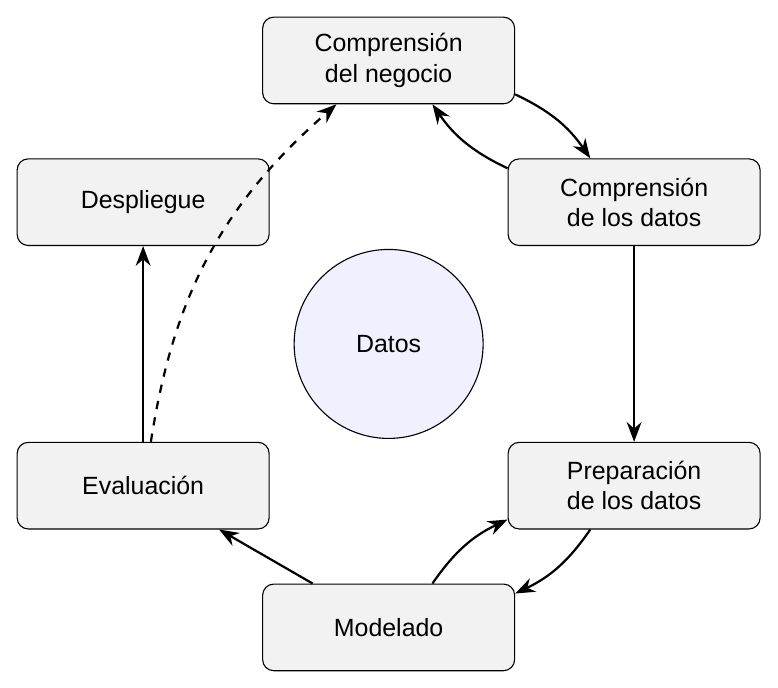
\includegraphics[width=0.6\textwidth]{imagenes/06_marco_teorico/crisp_dm.png}
  \fuente{Adaptado de \textcite{chapman2000}.}
\end{figure}

Una característica central de CRISP-DM es su carácter iterativo: la secuencia de fases no es
rígida, y el modelo contempla de forma explícita el retorno a fases anteriores cuando los
hallazgos lo requieren, por ejemplo cuando la exploración de los datos obliga a reformular
el objetivo o cuando el modelado revela la necesidad de nuevas variables. El ciclo externo
del diagrama de referencia (figura~\ref{fig:crisp-dm}) expresa, además, que el propio proceso
de minería de datos continúa tras el despliegue, porque las lecciones aprendidas generan
nuevas preguntas. La guía de referencia reconoce también que la preparación de los datos
suele concentrar la mayor parte del esfuerzo de un proyecto, un rasgo que se acentúa en
proyectos geoespaciales que integran fuentes heterogéneas.

CRISP-DM no es el único marco disponible. El proceso de descubrimiento de conocimiento en
bases de datos (KDD), descrito por \textcite{fayyad1996}, organiza el trabajo en etapas de
selección, preprocesamiento, transformación, minería de datos e interpretación o evaluación,
con un énfasis mayor en el proceso técnico de extracción de patrones que en la comprensión
del negocio. SEMMA, propuesto por SAS Institute, estructura el trabajo en las etapas de
muestreo, exploración, modificación, modelado y evaluación (\textit{Sample, Explore, Modify,
Model, Assess}), y está estrechamente asociado a las herramientas de ese proveedor. Frente a
ambos, CRISP-DM se distingue por incorporar explícitamente la comprensión del negocio y el
despliegue. En años recientes se han propuesto extensiones: \textcite{martinez2021}
analizaron la vigencia de CRISP-DM veinte años después de su creación y propusieron un marco
de trayectorias de ciencia de datos que reconoce que los proyectos actuales no siempre
siguen un ciclo lineal orientado a un modelo, sino recorridos exploratorios diversos; y
\textcite{studer2021} formularon CRISP-ML(Q), un modelo de proceso para aplicaciones de
aprendizaje automático con una metodología de aseguramiento de la calidad, que abarca seis
fases desde la definición del alcance hasta el mantenimiento de la aplicación desplegada,
ejecuta simultáneamente la comprensión del negocio y la de los datos, e incorpora de forma
explícita el monitoreo y el mantenimiento del modelo en operación frente a riesgos como la
deriva de los datos.

Se adopta CRISP-DM en este proyecto por su amplia aceptación en la práctica y en la
formación académica, por su énfasis en la comprensión del problema de la organización
destinataria y por su compatibilidad con las extensiones de CRISP-ML(Q) para la fase de
despliegue. Conforme a esta metodología, el proyecto se estructura de la siguiente manera.
En la comprensión del negocio se define el problema de los voluntarios de la Trufi
Association, que consiste en priorizar dónde revisar o mapear rutas, y se traduce en el
estimando del proyecto: el número esperado de consultas de cada zona dada su población y su
contexto territorial, cuyo contraste con lo observado orienta la priorización. En la
comprensión de los datos se exploran las consultas semanales y su distribución espacial y
temporal, se caracteriza el período sin datos de siete semanas, se examinan las ediciones de
población de Kontur y el feed GTFS de Trufi, y se analiza la autocorrelación espacial de las
consultas. En la preparación de los datos se depuran las consultas, se asignan a zonas H3 de
resolución~8, se integran con la población y con la cobertura medida como distancia al
trazado, y se construyen las macrozonas de resolución~6 que sirven como bloques de
validación. En el modelado se compara la escalera de técnicas descrita en
\ref{sec:tecnicas-algoritmos} mediante validación cruzada espacial por bloques. En la
evaluación se aplica una única vez el conjunto de prueba reservado, se calculan las métricas
descritas en \ref{sec:metricas}, se aplica la regla de selección declarada de antemano y se
realizan los análisis de sensibilidad y de estabilidad de la priorización. Finalmente, el
despliegue se limita a una propuesta de pipeline reproducible de actualización, que permita
reejecutar el proceso con nuevas consultas y nuevas ediciones de población y monitorear la
deriva de los datos al estilo de CRISP-ML(Q), junto con los entregables del proyecto, que
son un mapa interactivo, un archivo de estimaciones por zona y una lista de zonas
prioritarias para revisión, sin implementación operativa en los sistemas de Trufi.
